\chapter{DNS}
\label{chap:dns}
DNS bietet ein Service zur standardisierten Auflösung von Ressourcennamen innerhalb globaler oder lokaler Computernetzwerke \cite{rfc1035}. Dabei werden menschenlesbare Zeichenketten (Namen) in Adressen übersetzt. Des Weiteren ist es möglich, zusätzliche Informationen über diese Namen vom System abzufragen.

\section{Aufbau des DNS}
DNS ist als globale Datenbank mit Baum-Struktur konzipiert, welche über eine beliebige Anzahl an vernetzten Rechnern verteilt wird. Der Wurzelknoten des Baums wird dabei als Root bezeichnet und von der \ac{IANA} betrieben. Die Daten dieses Root-Knotens werden über 13 global verteilte Server bereitgestellt. 

Knoten der darunterliegenden und damit ersten Ebene werden als \acp{TLD} bezeichnet und sind nach Ländern (Country-Code TLD; ccTLD) oder Verwendung (Generic TLD; gTLD) gruppiert. Da manche Funktionen von DNS spezielle Domänen benötigen, existiert eine gesonderte Infrastruktur-\ac{TLD} (.arpa) die direkt von der \ac{IANA} verwaltet wird. Die anderen TLDs werden von verschiedenen Institutionen betrieben und stellen die höchste Stufe der DNS-Hierarchie dar. Diese sind für die Weitergabe der Verwaltungsrechte der ihnen nachfolgende Unterdomänen, sogenannte \acp{SLD}, verantwortlich. Will eine Person das Recht zur Verwaltung einer \ac{SLD} erhalten, muss dies über einen Antrag bei der verwaltenden Stelle oder eines berechtigten Subkontraktors erfolgen. Ist die gewünschte Domäne, z.B. example.com, noch nicht vergeben, werden die Verwaltungsberechtigungen, gegen eine Gebühr, in den Besitz der Antragstellenden übergehen. Alle untergeordneten Domänen sind damit ebenfalls in deren Verantwortung übergegangen. Dieser Aufbau führt zu einer schichtweisen Delegation der Aufgaben innerhalb des globalen DNS-Namensraums (siehe Abb. \ref{img:dnsnamespace}). 

\begin{figure}[!hb]
    \centering
    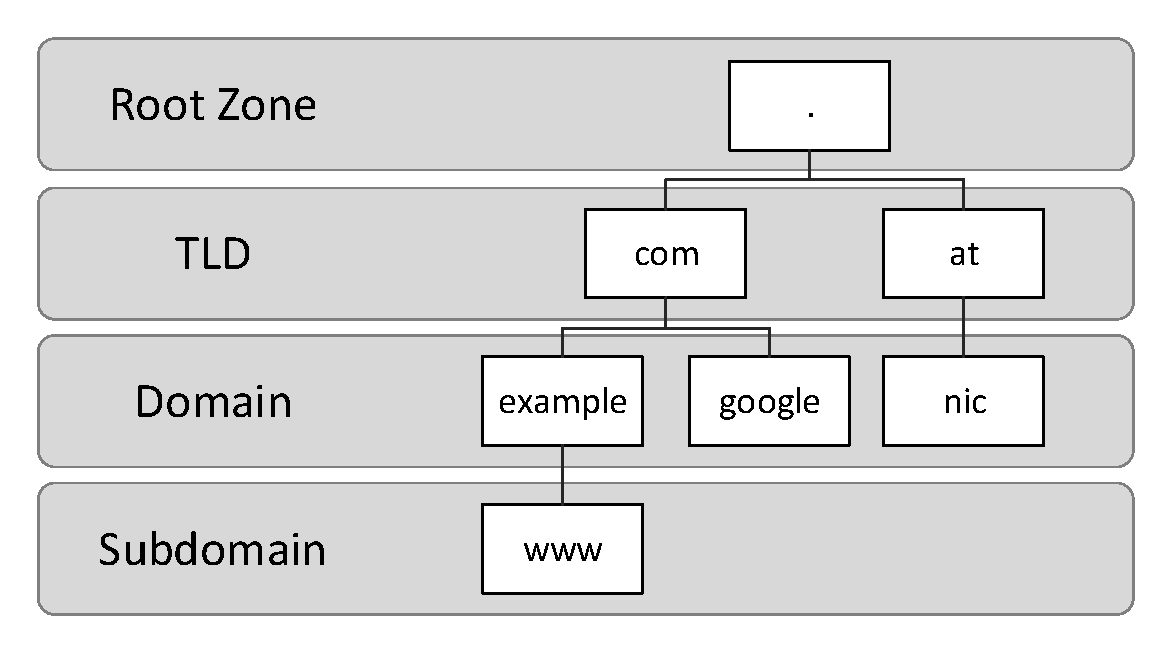
\includegraphics[width=0.5\textwidth]{DNS_NameSpaceLayers}
    \caption{Aufbau des DNS}
    \label{img:dnsnamespace}
\end{figure}

\section{Ressource Records, Sets und Zonen}
Alle Datensätze in DNS werden in einer als \ac{RR} bezeichneter Datenstruktur abgelegt. Ein \ac{RR} besteht aus 5 Informationen: Namen, \ac{TTL}, Klasse (Class), Typ (Type), Datenfeld (Data). Die Felder \ac{TTL} und Class sind optional. Die Menge an Einträgen mit gleichen Werten der Felder Name, TTL, Class und Type bilden ein \ac{RRset}\cite{rfc2181}, das kleinstmögliche abfragbare Element in DNS. Alle \ac{RR} die einem definierten, zusammenhängenden Teil des DNS Namensraum zugeordnet sind, werden als Zone bezeichnet. Diese Sammlung an RR wird in einer Datei, dem \textit{Zone File}, gespeichert und von DNS-Server-Implementationen als Datenbasis genutzt.   

Wie in Listing \ref{lst:dnsZoneFile} zu sehen ist, werden die Daten in einem menschenlesbaren Format gespeichert. Zeile 1 enthält die Anweisung den Namens \texttt{test.example.com.} zu den IPv4-Adressen \texttt{172.30.0.7} und \texttt{172.30.0.8} aufzulösen. Zeile 3 fügt dem Namen weiter Information im Freitextformat hinzu. Zeile 1 und 2 bilden zusammen ein RRset für \texttt{test.example.com 3600 IN A}.

\lstinputlisting[caption={Ausschnitt aus dem Zone-File \textit{example.com}}, label={lst:dnsZoneFile}]{code/example-zone.txt}

\section{DNS Server}
\label{sec:dnsserver}
Um die globale, verteilte Datenbank des DNS nutzen zu können, ist es notwendig, dass diese den DNS-Client-Programmen zugänglich gemacht wird. Das Netzwerkprotokoll ist nach dem klassischen Client-/Server-Konzept ausgestaltet. Es erfordert keinen Verbindungsaufbau und verwendet einen einfachen, sequenziellen Ablauf an Anfragen und Antworten. Ein Client stellt immer nur Anfragen an Server und verarbeitet deren Antwort. DNS-Server können hingegen, je nach Typ, selbst Anfragen an andere Server stellen und sind somit nicht auf das Beantworten von Anfragen beschränkt. Es können insgesamt vier unterschiedliche DNS-Server-Typen festgemacht werden.

\paragraph{Stub Resolver}
Die Software, die auf jedem Client-Rechner DNS-Anfragen von Programmen entgegennimmt und diese an die DNS Infrastruktur zur Auflösung übergibt, werden als \textit{Stub Resolver} (auch Stub) bezeichnet. Diese können nach außen ausschließlich mit rekursiven Resolvern kommunizieren und nehmen selbst keine DNS-Namensauflösung vor. In manchen Fällen verfügen sie hingegen über einen Cache oder können aufgrund lokaler Policies (z.B. einem Hosts-File) eine Namensauflösung auf anderem Wege durchführen.

\paragraph{Rekursive Resolver}
\textit{Recursive Resolver} sind spezielle DNS-Server die von Clients genutzt werden, um Namen aufzulösen. Sie verfügen meistens über keine eigenen Zonen und sind damit als Vermittlungskomponente zwischen Endgeräten und den im Internet verfügbaren DNS-Servern zu verstehen.

\paragraph{Autoritative Server}
Server deren Hauptaufgaben im Auflösen von Namen einer oder mehrerer bestimmter Zonen besteht, werden \textit{autoritative Server} genannt. Die Bezeichnung spielt auf den Umstand an, dass die Antworten dieses Servers die finale Wahrheit über die von ihm verwalteten Zonen darstellt. Sie lesen die Antworten direkt auf dem Zonen-File der entsprechenden Zone und verlassen sich nicht auf Antworten anderer Server oder Caches. Autoritative DNS-Server stellen damit die Endpunkte der Auflösung für die jeweiligen Domänen dar.

\paragraph{Forwarding DNS Server}
Eine spezielle Form des Rekursive Resolver wird als \textit{Forwarding DNS Server} oder \textit{Forwarding Resolver} bezeichnet. Aus Sicht des Stub Resolvers verhält er sich wie ein gewöhnlicher Rekursiver Resolver. Der Unterschied besteht darin, dass er selbst keinen Auflöse-Prozess durchführt. Die Anfragen werden lediglich an einen anderen Server weiterleitet, welcher die eigentliche Auflösung durchführt. Die Ergebnisse werden meist gecacht bevor sie an den Client weitergegeben werden.

\section{DNS Namensauflösungsprozess}
\label{sec:dnsresolution}
Der Namensauflösungsprozess erfolgt über mehrere Schritte und kann am besten anhand eines Beispiels dargestellt werden. Nehmen wir an, eine Applikation möchte die IPv4-Adresse des Namen \texttt{example.com} herausfinden und stellt eine Anfrage an den lokalen Stub Resolver des Client. Der Prozess ist in Abb. \ref{img:dnsresolution} visualisiert und kann Schrittweise wie folgt beschrieben werden:

\begin{enumerate}
    \item Der Stub stellt eine Anfrage nach dem A Record der Domäne example.com an den für ihn konfigurierten rekursiven Resolver.
    \item Der Resolver empfängt die Anfrage und prüft seinen lokalen Cache nach dem Eintrag. Da er diesen nicht auffindet, wird fortgefahren.
    \item Nun startet der Resolver den rekursiven Auflösungsvorgang. Geht man von einem leeren Cache aus, wird mit der Root-Zone (.) begonnen. Die Anfrage nach www.example.com wird dafür an einen der 13 vorkonfigurierten Root-DNS-Server gesendet.
    \item Der Root-Server empfängt die Anfrage, kann jedoch nur den TLD Teil der Antwort auflösen. Es sendet daher die Adressen des autoritativen Nameserver für die TLD .com zurück.
    \item Der Resolver verarbeitet die Adressen und sendet die Anfrage an einen der autoritativen Server der .com Domäne.
    \item Der TLD Nameserver empfängt die Anfrage und prüft, ob für die Domäne example.com eine entsprechende Delegation existiert. Da diese in Form mehrerer NS Einträge vorliegt, wird eine Liste an autoritativen Nameserver-Adressen der SLD Domäne example.com als Antwort gesendet.
    \item Da die Adresse eines autoritative Servers für Zieldomäne example.com gefunden wurde, kann die gewünschte Information abgefragt werden. Der Resolver sendet also ein letztes mal die Anfrage des Client, jetzt an den Nameserver der SLD example.com.
    \item Der autoritative Server der SDL example.com nimmt die Anfrage nach dem RR mit Typ A für die Domäne example.com entgegen und liefert nun die gewünschte Information in Form einer IPv4 Adresse.
    \item Der rekursive Resolver empfängt die Antwort, überträgt sie in seinen Cache und sendet dem anfragenden Stub die IPv4 Adresse zurück.
\end{enumerate}

\begin{figure}[htbp]
    \centering
    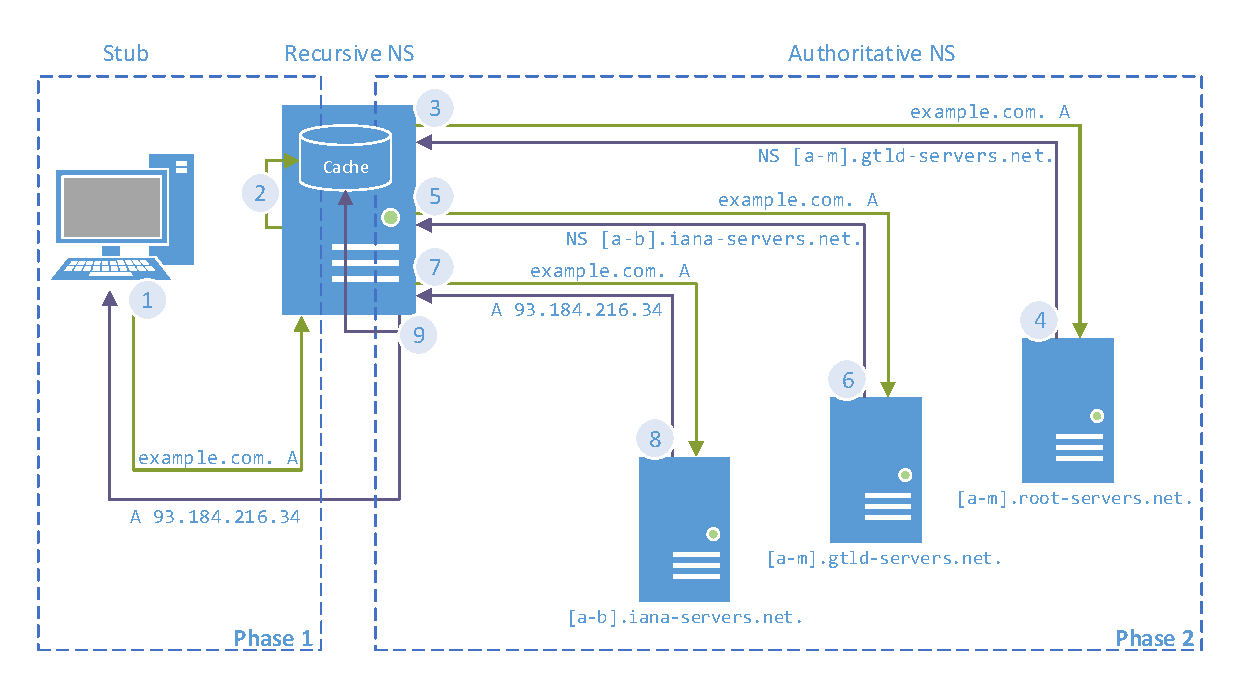
\includegraphics[width=\textwidth]{DNS_Resolution}
    \caption[Dargestellte des DNS Auflösungsprozess für \texttt{example.com}]{Der schrittweise dargestellte Auflösungsprozess des Namen \texttt{example.com} über DNS. Der zeitliche Ablauf wird über die nummerierten Markierungen angezeigt.}
    \label{img:dnsresolution}
\end{figure}

\section{DNS Security}
\label{sec:dnssecurity}
Obwohl oder gerade weil DNS eines der grundlegendsten Services im Internet darstellt, wurde bei der Spezifikation des Netzwerkprotokolls bewusst auf eine Authentifizierung verzichtet. Dies ist auf die Idee einer öffentlich zugänglichen, globalen Datenbank, nach dem Vorbild eines globalen Telefonregisters, zurückzuführen. Die Datenbasis der Namensauflösung wurde somit als frei öffentlich zugänglich definiert \cite{rfc1035}. Abgesehen davon stammt das Protokoll aus einer Zeit, in der modernen Schutzzielen, wie Sicherheit und Vertraulichkeit wenig Beachtung geschenkt wurde. Dies führt zu einer Vernachlässigung des Sicherheitsgedanken und hat sich über die Zeit zu einem ernstzunehmenden Problem entwickelt. Verschärfend kommt hinzu, dass kein allgemeiner Konsens über die Sicherheitsziele herrscht. Dies erschwert die Entwicklung einer Lösung und hat zu den unterschiedlichsten Ansätzen und Technologien geführt \cite{Grothoff2018}.

\section{Resolver Position}
\label{sec:dnsresolverposition}
Der Aufbau der Client-nahen Infrastruktur spielt eine wichtige Rolle für die Sicherheit des Clients. Wie im Abschnitt \ref{sec:dnsresolution} beschrieben, wird vom Client ein Recursive Resolver benötigt, um die eigentliche Auflösung der Namen durchzuführen. Die Lage dieser Komponente im Netzwerk ist vor allem für Privacy ausschlaggebend. Es existieren insgesamt fünf mögliche Positionen die ein Recursive Resolver einnehmen kann \cite{VanHeugten2018} (siehe Abbildung \ref{img:dnsresolverposition}):

\paragraph{Local Recursive Resolver}
Ist der Recursive Resolver im Netzwerk des Clients positioniert und wird die selbe öffentliche IP-Adresse zur externen Kommunikation benützt, spricht man von einem \textit{Local Recursive Resolver}. Da dieser in den meisten Fällen unter der Kontrolle des Benutzers steht und nicht von Dritten überwacht wird, ist es unbedenklich, dass Anfrage und Client-IP einfach ausgelesen werden können. Da für die gesamte internet-gerichtete Kommunikation, inklusive des rekursiven Auflöseprozesses, die selbe Adresse verwendet wird, ist es für Betreiber von Zwischenstellen einfach eine Verbindung zwischen Anfrage und User herzustellen \cite{Shulman2014}.

\paragraph{Private Recursive Resolver}
Unter \textit{Private Recursive Resolver} können alle Resolver zusammengefasst werden, die zwar unter der Kontrolle der nutzenden Personen stehen, aber nicht die selbe Adresse für die Kommunikation verwendet. Da die autoritativen DNS-Server von der Resolver-Adresse aus angesprochen werden, ist keine Verknüpfung zur Client-Adresse mehr möglich. Dies hilft der Privacy hingegen nur, wenn die Adresse des Servers nicht trotzdem einer einzelnen Person zugeordnet werden kann.

\paragraph{ISP Recursive Resolver}
Die Mehrheit der Nutzenden im privaten oder einzelunternehmerischen Umfeld verwenden den Resolver ihres \ac{ISP}. Diese \textit{ISP Recursive Resolver} werden von den Internetanbietern zur Verfügung gestellt, um eine grundlegende Internetkonnektivität anbieten zu können. Diese Server sind in den meisten Fällen im Netzwerk des ISP positioniert und haben daher oft bessere Latenzzeiten als andere, über das Internet erreichbare, Resolver. Diese Resolver werden oft für das Überwachen von Kundenaktivitäten und einspeisen von Werbeseiten verwendet \cite{Weaver2011}, was grundsätzlich gegen den Gedanken der Privacy verstößt.

\paragraph{Public Recursive Resolver}
Sogenannte \textit{Public Recursive Resolver} sind über ihre freie Zugänglichkeit definiert und haben je nach Fokus des Anbieters verschiedenste Regelungen was Privacy betrifft \cite{Prince2018}\cite{Quad92018}. Wird ein Anbieter mit speziellem Fokus auf Sicherheit und Vertraulichkeit gewählt, kann ein akzeptabler Grad an Privacy erreicht werden. Voraussetzung dafür ist die Sicherung der Übertragung zwischen Stub-Resolver und Recursive Resolver. Einige Projekte bieten dafür Unterstützung spezielle Netzwerkprotokolle, die diesen Zweck erfüllen sollen (siehe dazu Kapitel \ref{chap:technologies}). Resolver die speziellen, selbst auferlegten Vorschriften zur Verbesserung der Informationssicherheit folgen, werden als \textit{Trusted Resolver} bezeichnet, wobei diese öffentlich (public) oder nur mit Authentifizierung (private) zugänglich sein können.

\paragraph{Local-Loopback Resolver}
Eine Sonderform stellt der \textbf{Local-Loopback Resolver} dar. Dieser wird direkt auf dem Client-Rechner installiert und ist nur für Programme auf eben diesem Host erreichbar. Dies führt zu dem Umstand, dass der Stub-Resolver keine für das umliegende Netzwerk sichtbare Kommunikation mehr durchführt. Der Installierte Resolver löst die Anfragen dann entweder rekursiv über das Netzwerk auf oder fungiert als Forwarding Resolver (siehe Abschnitt \ref{sec:dnsserver}) und verhält sich somit wie ein Stub-Resolver.

\begin{figure}[htbp]
    \centering
    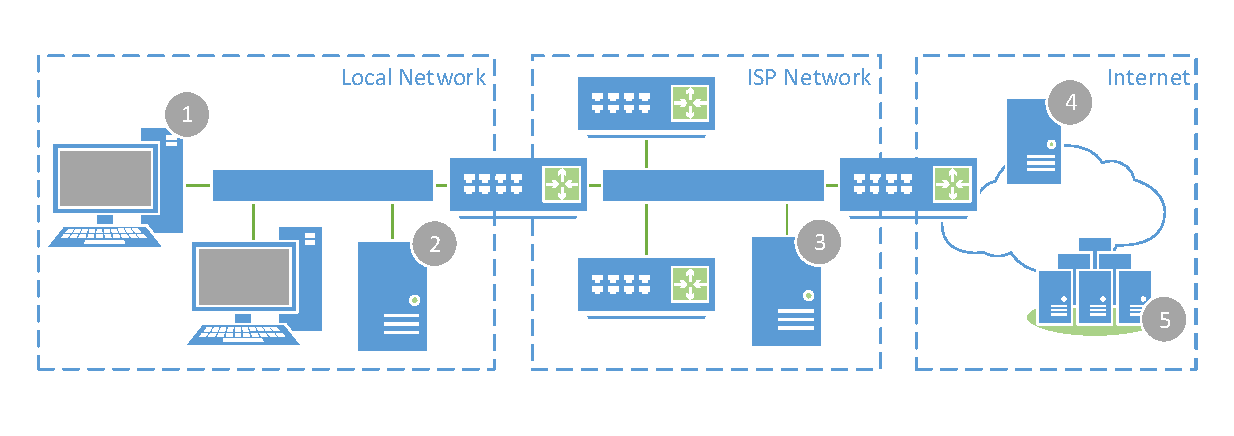
\includegraphics[width=\textwidth,trim={0 1cm 0 0.5cm},clip]{DNS_ResolverPosition}
    \caption[Darstellung möglicher DNS-Resolver positionen im Netzwerk]{Zeigt die möglichen Positionen eines DNS-Resolvers in einem herkömmlichen Netzwerkaufbau mit Internetzugang. (1) Local-Loopback Resolver, (2) Local Recursive Resolver, (3) ISP Recursive Resolver, (4) Private Recursive Resolver, (5) Public Resolver}
    \label{img:dnsresolverposition}
\end{figure}
